% Format teze zasnovan je na paketu memoir
% http://tug.ctan.org/macros/latex/contrib/memoir/memman.pdf ili
% http://texdoc.net/texmf-dist/doc/latex/memoir/memman.pdf
% 
% Prilikom zadavanja klase memoir, navedenim opcijama se podešava 
% veličina slova (12pt) i jednostrano štampanje (oneside).
% Ove parametre možete menjati samo ako pravite nezvanične verzije
% mastera za privatnu upotrebu (na primer, u b5 varijanti ima smisla 
% smanjiti 
\documentclass[12pt,oneside]{memoir} 

% Paket koji definiše sve specifičnosti master rada Matematičkog fakulteta
\usepackage[latinica,biblatex]{matfmaster} 
%
% Podrazumevano pismo je ćirilica.
%   Ako koristite pdflatex, a ne xetex, sav latinički tekst na srpskom jeziku
%   treba biti okružen sa \lat{...} ili \begin{latinica}...\end{latinica}.
%
% Opicija [latinica]:
%   ako želite da pišete latiniciom, dodajte opciju "latinica" tj.
%   prethodni paket uključite pomoću: \usepackage[latinica]{matfmaster}.
%   Ako koristite pdflatex, a ne xetex, sav ćirilički tekst treba biti
%   okružen sa \cir{...} ili \begin{cirilica}...\end{cirilica}.
%
% Opcija [biblatex]:
%   ako želite da koristite reference na više jezika i umesto paketa
%   bibtex da koristite BibLaTeX/Biber, dodajte opciju "biblatex" tj.
%   prethodni paket uključite pomoću: \usepackage[biblatex]{matfmaster}
%
% Opcija [b5paper]:
%   ako želite da napravite verziju teze u manjem (b5) formatu, navedite
%   opciju "b5paper", tj. prethodni paket uključite pomoću: 
%   \usepackage[b5paper]{matfmaster}. Tada ima smisla razmisliti o promeni
%   veličine slova (izmenom opcije 12pt na 11pt u \documentclass{memoir}).
%
% Naravno, opcije je moguće kombinovati.
% Npr. \usepackage[b5paper,biblatex]{matfmaster}

% Pomoćni paket koji generiše nasumičan tekst u kojem se javljaju sva slova
% azbuke (nema potrebe koristiti ovo u pravim disertacijama)
\usepackage[latinica]{pangrami}

% Datoteka sa literaturom u BibTex tj. BibLaTeX/Biber formatu
\bib{DjordjeTodorovicMasterRad}

\newtheorem{primer}{Primer}

% Ime kandidata na srpskom jeziku (u odabranom pismu)
\autor{Đorđe Todorović}
% Naslov teze na srpskom jeziku (u odabranom pismu)
\naslov{Podrška za naprednu analizu promenljivih lokalnih za niti pomoću alata GNU GDB}
% Godina u kojoj je teza predana komisiji
\godina{2018}
% Ime i afilijacija mentora (u odabranom pismu)
\mentor{dr Mika \textsc{Mikić}, redovan profesor\\ Univerzitet u Beogradu, Matematički fakultet}
% Ime i afilijacija prvog člana komisije (u odabranom pismu)
\komisijaA{dr Ana \textsc{Anić}, vanredni profesor\\ University of Disneyland, Nedođija}
% Ime i afilijacija drugog člana komisije (u odabranom pismu)
\komisijaB{dr Laza \textsc{Lazić}, docent\\ Univerzitet u Beogradu, Matematički fakultet}
% Ime i afilijacija trećeg člana komisije (opciono)
% \komisijaC{}
% Ime i afilijacija četvrtog člana komisije (opciono)
% \komisijaD{}
% Datum odbrane (odkomentarisati narednu liniju i upisati datum odbrane ako je poznat)
% \datumodbrane{}

% Apstrakt na srpskom jeziku (u odabranom pismu)
\apstr{%

}

% Ključne reči na srpskom jeziku (u odabranom pismu)
\kljucnereci{analiza, geometrija, algebra, logika, računarstvo, astronomija}

\begin{document}
% ==============================================================================
% Uvodni deo teze
\frontmatter
% ==============================================================================
% Naslovna strana
\naslovna
% Strana sa podacima o mentoru i članovima komisije
\komisija
% Strana sa posvetom (u odabranom pismu)
\posveta{Mami, tati i dedi}
% Strana sa podacima o disertaciji na srpskom jeziku
%\apstrakt
% Sadržaj teze
\tableofcontents*

% ==============================================================================
% Glavni deo teze
\mainmatter
% ==============================================================================

% ------------------------------------------------------------------------------
\chapter{Uvod}
% ------------------------------------------------------------------------------

% ------------------------------------------------------------------------------

\chapter{Kako rade debageri?}
\label{chp:debageri}

Greške su sastavni deo svakog rada koji obavlja čovek, te ih i programeri prave. Greške mogu biti hardverske i softverske. One mogu imati razne poslednice. Neke su manje važne, kao npr.~korisnički interfejs aplikacije ima neočekivanu boju pozadine. Postoje i greške koje mogu imati daleko veće posledice, pa čak i ugroziti živote drugih, kao npr.~greške u softveru ili hardveru uređaja i aplikacija avio industrije. Faza testiranja je veoma važna u ciklusu razvoja softvera. Nakon faze testiranja obično sledi faza analize i otklanjanja grešaka.

Debager (eng.~\emph{debagger}) je softverski alat koji koriste programeri za testiranje, analizu i otklanjanje grešaka u programima. Sam proces korišćenja takvih alata nazivamo debagovanjem (eng.~\emph{debugging}).
Debageri mogu pokrenuti rad nekog procesa ili se „nakačiti” na proces koji je već u fazi rada. U oba slučaja, debager preuzima kontrolu nad procesom. To mu mogućava da izvršava proces instrukciju po instrukciju, do postavlja tačke prekida (eng.~\emph{brakpoints}) itd. Proces izvršavanja programa od strane debagera sekvencijalno, instrukciju po instrukciju ili liniju po liniju, nazivamo koračanje. Tačke prekida su mogućnost debagera da zaustavi izvršavanje programa na određenoj tački. To može biti trenutak kada program izvrši određenu funkciju, liniju koda itd. Neki debageri imaju mogućnost izvršavanja funkcija programa koji se debaguje, uz ograničenje da program pripada istoj procesorskoj arhitekturi kao i domaćinski sistem na kojem se debager izvršava. Čak i struktura programa može biti promenjena, prateći propratne efekte.

Podršku debagerima, u opštem slučaju, daju operativni sistemi, kroz sistemske pozive koji omogućavaju tim alatima da pokrenu i preuzmu kontrolu nad nekim drugim procesom. Za neke naprednije tehnike debagovanja poželjna je podrška od strane hardvera. U radu će detaljno biti obrađen rad UNIX-olikih, posebno Linux debagera. Windows debageri i programski prevodioci ne prate standard DWARF \cite{DWARF} prilikom baratanja sa debag informacijama namenjene za taj operativni sistem. Alati za debagovanje u okviru operativnog sistema Windows koriste standard \emph{Majkrosoft CodeView}.  Više informacija o ovom standardu može se pronaći u literaturi \cite{CodeView}.

\section{Prevođenje programa}

Programi koji se debaguju se prevode uz pomoć odgovarajuće opcije programskih prevodioca (za prevodioce GCC i LLVM/Clang, to je opcija \texttt{-g}) koja obezbeđuje generisanje pomoćnih debag informacija. Ukoliko je program koji se analizira preveden bez optimizacija, debag informacije koje prate program su potpune. Programi koji se puštaju u produkciju, da bi bili brži i zauzimali manje memorije, se prevode uz pomoć optimizacija. Nivoi optimizacija produkcijskih programa su "-O2" i "-O3". Prilikom optimizacija se gube razne debag informacije. Neke promenljive i funkcije programa neće biti predstavljene debag informacijama. Npr.~ promenljiva programa može biti živa samo u nekim određenim delovima programa, pa programski prevodioci generišu debag informacije o njenim lokacijama samo u tim određenim delovima koda. Prilikom optimizacija na nivou mašinskog koda život promenljive može biti skraćen, pa čitanje vrednosti promenljive iz debagera u nekim sitacijama neće biti moguće, iako gledajući izvorni kod očekujemo da je ona živa u tom trenutku.

\section{Fajl format DWARF}

DWARF je debag fajl format koji se koristi od strane programskih prevodioca (kao npr.~GCC ili LLVM/Clang) i debagera (kao npr.~GNU GDB) da bi se omogućilo debagovanje na nivou izvornog koda. Omogućava podršku za razne programske jezike kao što su C/C++ i Fortran, ali je dizajniran tako da se lako može proširiti na ostale jezike. Arhitekturalno je nezavisan i predstavlja "most" između izvornog koda i izvršnog fajla. Trenutno je poslednji realizovani standard verzija 5 formata DWARF.

Debag fajl format DWARF se odnosi na Unix-olike operativne sisteme, kao što su Linux i MacOS. Generisane debag informacije, prateći DWARF standard, su podeljene u nekoliko sekcija sa prefiksom \texttt{.debug\_}. Neke od njih su \texttt{.debug\_line}, \texttt{.debug\_loc} i \texttt{.debug\_info} koje redom predstavljaju informacije o linijama izvornog koda, lokacijama promenljivih i ključna debag sekcija koja sadrži debag informacije koje referišu na informacije iz ostalih debag sekcija.
DWARF je predstavljen kao drvolika struktura, smeštena u \texttt{.debug\_info} sekciju,  koja razne entitete programskog jezika opisuje osnovnom debag jedinicom DIE (eng.~Debug Info Entry). Osnovna debag jedinica može opisivati lokalnu promenljivu programa, formalni parametar, funkciju itd. Svaka od njih je identifikovana DWARF tagom koji predstavalja informaciju o toj jedinici, gde je npr.~tag za lokalne promenljive predstavljen sa \texttt{DW\_TAG\_local\_variable}, ili tag za funkciju je obeležen sa \texttt{DW\_TAG\_subprogram}. Svaka debag jedinica je opisana određenim DWARF atributima sa prefikosm \texttt{DW\_AT\_}. Oni mogu ukazivati na razne informacije o entitetu kao sto su ime promenljive ili funkcije, liniju deklaracije, itd. Koren svakog DWARF stabla je predstavljen debag jedinicom, sa tagom  \texttt{DW\_TAG\_compile\_unit}, koja predstavlja kompilacionu jedinicu, tj. izvorni kod programa. Primer dela DWARF stabla za primer predstavljen slikom \ref{fig:testPrimer} je dat slikom \ref{fig:dwarfPrimer}.

\begin{figure}[h!]
	\begin{center}
		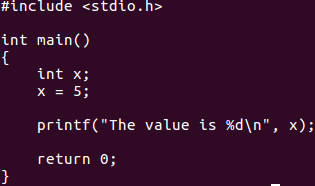
\includegraphics[scale=0.8]{slike/testPrimer.png}
	\end{center}
	\caption{Izvorni k\^{o}d test primera koji se analizira.}
	\label{fig:testPrimer}
\end{figure}

\begin{figure}[h!]
	\begin{center}
		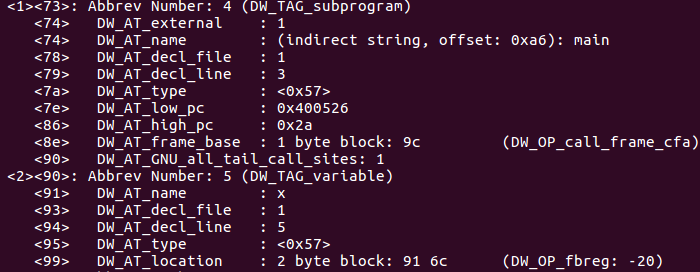
\includegraphics[scale=0.6]{slike/dwarfPrimer.png}
	\end{center}
	\caption{Debug jedinice DWARF stabla primera sa slike \ref{fig:testPrimer}.}
	\label{fig:dwarfPrimer}
\end{figure}

Funkcija \texttt{main} primera sa slike \ref{fig:testPrimer} na slici \ref{fig:dwarfPrimer} je predstavljena DWARF tagom \texttt{DW\_TAG\_subprogram}. Atribut te debag jedinice predstavljen sa \texttt{DW\_AT\_name} ima vrednost imena funkcije. Atributi \texttt{DW\_AT\_low\_pc} i \texttt{DW\_AT\_high\_pc} redom predstavljaju adresu prve mašinske instrukcije te funkcije u memoriji programa i ofset na kojem se nalazi poslednja mašinska instrukcija te funkcije. Sledeći čvor drveta predstavlja promenljivu \texttt{x} istog test primera. Ta debag jedinica je dete čvora koji predstavlja funkciju \texttt{main} i ukazuje da se promenljiva \texttt{x} nalazi unutar funkcije \texttt{main}. Promenljiva \texttt{x} je predstavljena DWARF tagom \texttt{DW\_TAG\_variable}. Atribut \texttt{DW\_AT\_name} predstavlja ime promenljive, \texttt{DW\_AT\_type} referiše na debag jedinicu koja predstavlja tip promenljive, dok \texttt{DW\_AT\_location} atribut predstavlja lokaciju promenljive u memoriji programa. 

\subsection{Debag promenljive}

Svaka promenljiva programa prevedenog sa debag informacijama, ukoliko se ne radi o optimizovanom programu, je predstavljena DWARF tagom \texttt{DW\_TAG\_variable}. Atribut \texttt{DW\_AT\_location} ukazuje na lokaciju promenljive. Lokacija može biti predstavljena DWARF izrazom, kao npr.~lokacija promenljive \texttt{x} na slici \ref{fig:dwarfPrimer}. DWARF izraz te promenljive ukazuje da se ona nalazi na ofsetu -20 trenutnog stek okvira \texttt{main} funkcije. U neoptimizovanom kodu sve promenljive imaju lokacije zadate DWARF izrazom. Njihove vrednosti su dostupne debagerima u bilo kom delu koda u kom su definisane.

U optimizovanom kodu lokacija promenljive može sadržati referencu na informaciju o lokaciji u \texttt{.debug\_loc} sekciji. Lokacije u toj sekciji su predstavljene listama lokacija. Jedna promenljiva u optimizovanom kodu može biti smeštena na raznim memorijskim lokacijama ili registrima. Elementi liste opisuju lokacije promenljive na mestima u kodu gde je ona živa. Ukoliko promenljiva nije živa u nekom delu koda, programski prevodioci u optimizovanom kodu neće pratiti njenu lokaciju. Slika \ref{fig:optPrimer} predstavlja primer lokacije promenljive u optimizovanom kodu.

\begin{figure}[h!]
	\begin{center}
		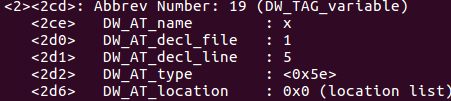
\includegraphics[scale=0.6]{slike/optimizovanPrimer.png}
	\end{center}
	\caption{Debag jedinica promenljive \texttt{x} u optimizovanom kodu.}
	\label{fig:optPrimer}
\end{figure}

Lokacijska lista promenljive \texttt{x} je predstavljena na slici \ref{fig:debugLoc}. U ovom konkretnom primeru, promenljiva živi samo na jednom mestu. Potencijalno je mogla imati još elemenata lokacijske liste. \texttt{Offset} predstavlja informaciju gde se lokacijska lista određene promenljive nalazi u \texttt{.debug\_loc} sekciji. \texttt{Begin} i \texttt{End} predstavljaju informaciju od koje do koje adrese u programu važi data lokacija, tj.~od koje do koje instrukcije je određena promenljiva živa. \texttt{Expression} predstavlja DWARF izraz koji opisuje lokaciju promenljive.

\begin{figure}[h!]
	\begin{center}
		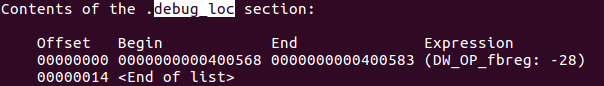
\includegraphics[scale=0.6]{slike/debugLoc.png}
	\end{center}
	\caption{Lokacijska lista promenljive \texttt{x} u optimizovanom kodu.}
	\label{fig:debugLoc}
\end{figure}

%\section{Linux debageri}
\newpage
\section{Fajl format ELF}

ELF (eng.~\emph{Executable and Linkable Format}) \cite{ELF} je format izvršnih fajlova, deljenih biblioteka, objektnih fajlova i datoteka jezgara.

ELF sadrži razne informacije o samom fajlu. Podeljen je u dva dela: ELF zaglavlje i podaci fajla. ELF zaglavlje sadrži informacije o arhitekturi za koju je program preveden i definiše da li program koristi 32-bitni ili 64-bitni adresni prostor. Zaglavlje 32-bitnih programa je dužine 52 bajta, dok kod 64-bitnih programa zaglavlje je dužine 64 bajta. Podaci fajla mogu sadržati programsku tabelu zaglavlja (eng.~\emph{Program header table}), sekcijsku tabelu zaglavlja (eng.~\emph{Section header table}) i ulazne tačke prethodne dve tabele. Slika \ref{fig:elf} prikazuje primer prikaza fajla u formatu ELF.

\begin{figure}[h!]
	\begin{center}
		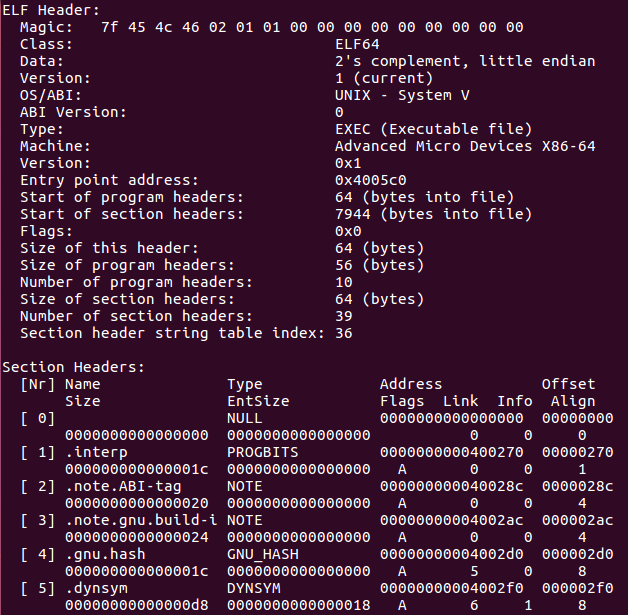
\includegraphics[scale=0.5]{slike/elf_example.png}
	\end{center}
	\caption{ELF fajl format počitan alatom \emph{objdump}.}
	\label{fig:elf}
\end{figure}

\section{Sistemski poziv \texttt{ptrace}}

Operativni sistem GNU Linux pruža sistemski poziv \texttt{ptrace} \cite{ptrace} koji debagerima omogućava rad. Ovaj sistemski poziv omogućava jednom procesu kontrolu nad izvršavanjem nekog drugog procesa i menjanje memorije i registara istog.
Potpis ove funkcije je:
\newline\newline
\texttt{ long ptrace\newline(enum \_\_ptrace\_request request, pid\_t pid, void *addr, void *data);}
\newline

Prvi argument sistemskog poziva predstavlja informaciju kojom operativnom sistemu jedan proces, ne nužno debager, ukazuje na nameru preuzimanja kontrole drugog procesa. Ukoliko taj argument ima vrednost \texttt{PTRACE\_TRACEME} to ukazuje na nameru praćenja (eng.~\emph{tracing}) određenig procesa, \texttt{PTRACE\_PEEKDATA} i \texttt{PTRACE\_POKEDATA} redom ukazuju na nameru čitanja i pisanja  memorije, \texttt{PTRACE\_GETREGS} i \texttt{PTRACE\_SETREGS} se odnose na čitanje i pisanje registara. To su samo neki osnovni slučajevi korišćenja, za više informacija pogledati \cite{ptrace}. Drugi argument sistemskog poziva \texttt{pid} ukazuje na identifikacioni broj ciljanog procesa. Treći i četvrti argument se po potrebi koriste u zavisnosti od namere korišćenja sistemskog poziva \texttt{ptrace} za čitanje ili pisanje sa adrese datom trećim argumentom, pri tom baratajući podacima na adresi zadatoj četvrtim argumentom. To znači ukoliko se koristi \texttt{PTRACE\_TRACEME} poslednja tri argumenta sistemskog poziva se ignorišu. Ukoliko se koristi \texttt{PTRACE\_GETREGS} sa adrese \texttt{addr} se čita jedna reč iz memorije. Navodimo par osnovnih primera korišćenja \texttt{ptrace} sistemskog poziva, a u nastavku će biti navedeno još primera.

\begin{primer}
Program inicira da će biti praćen od strane roditeljskog procesa:

\texttt{ptrace(PTRACE\_TRACEME, 0, NULL, NULL);}
\end{primer}

\begin{primer}
Čitanje vrednosti registara procesa sa identifikatorom \texttt{8845} i upisivanje tih vrednosti na adresu promenljive \texttt{regs}:

\texttt{ptrace(PTRACE\_GETREGS, 8845, NULL, \&regs);}

\end{primer}

\section{Realizacija osnovnih elemenata upotrebe debagera}

\subsection{Tačke prekida}

Postoje dve vrste tačaka prekida (eng.~\emph{breakpoints}): softverske i hardverske \cite{GDB}.

Osvrnimo se prvo na softverske tačke prekida. Postavljanje tačaka prekida predstavlja jednu od najkorišćenijih mogućnosti debagera, te stoga navedimo par smernica kako je ista realizovana, u opštem slučaju. Ali takođe treba napomenuti da ne postoji jedinstveni poziv nekog sistemskog poziva za postavljanje tačke prekida, već se ista obavlja kao kombinacija više mogućnosti  sistemskog poziva \texttt{ptrace}. Opišimo ceo postupak na jednostavnom primeru.

Program je preveden za procesorsku arhitekturu Intel x86-64 i asemblerski k\^{o}d \texttt{main} funkcije primera izgleda kao u primeru sa slike \ref{fig:primer1}.

\begin{figure}[h!]
	\begin{center}
		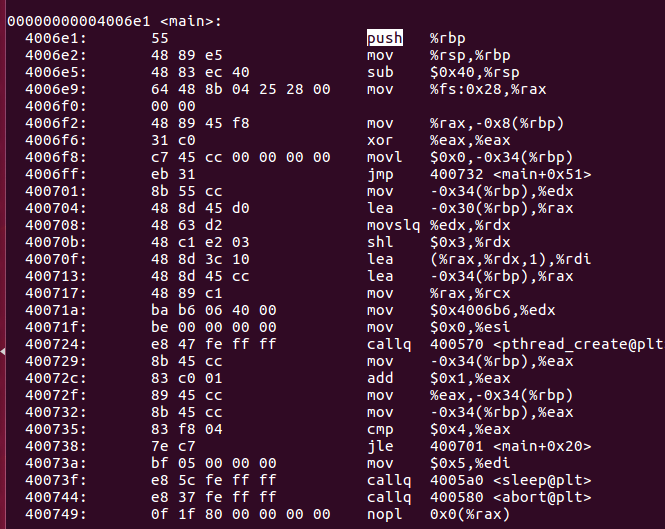
\includegraphics[scale=0.3]{slike/example_bp.png}
	\end{center}
	\caption{Asemblerski k\^{o}d \texttt{main} fukcije test primera na x86-64 platformi.}
	\label{fig:primer1}
\end{figure}

Primera radi, želimo da postavimo tačku prekida na treću po redu instrukciju funkcije \texttt{main}:

\texttt{48 89 e5  mov \%rsp,\%rbp}

Da bismo to uradili, menjamo prvi bajt instrukcije sa posebnom magičnom vrednošću, obično \texttt{0xcc}, i kada izvršavanje dostigne do tog dela koda ono će se zaustaviti na tom mestu.

Pošto \texttt{0x48} menjamo sa \texttt{0xcc} i na tom mestu u kodu dobijamo instrukciju:

\texttt{cc 89 e5  int3}

Ukoliko korisnik želi da nastavi dalje, instrukcija prekida se zamenjuje sa originalnom instrukcijom koja se izvršava i nastavlja se sa radom programa.

Instrukcija \texttt{int3} je posebna instrukcija procesorske arhitekture Intel x86-64, koja izazva softverski prekid. Kada registar programski brojač (eng.~\emph{CPU register pc}) stigne do \texttt{int3} instrukcije izvršavanje se zaustavalja na toj tački. Debager je već upoznat od strane korisnika da je tačka prekida postavljena te on čeka na signal koji ukazuje na to da je program dostigao do instrukcije prekida. Operativni sistem prepoznaje instrukciju \texttt{int3}, poziva se specijalni obrađivač tog signala (na Linux sistemima \texttt{do\_int3()}), koji dalje obaveštava debager šaljući mu signal sa kodom \texttt{SIGTRAP} koji on obrađuje na željeni način. Treba napomenuti da ovo važi za procesorsku arhitekturu Intel x86-64, instrukcija prekida za arhitekture kao što su ARM, MIPS, PPC itd., se drugačije kodira, ali postupak implementacije tačaka prekida je isti.

Ukoliko želimo da stavimo tačku prekida eksplicitno na funkciju \texttt{main}, za to koristimo posrednika u vidu DWARF debag informacija. U tom slučaju debager traži element DWARF stabla koji ukazuje na informacije o \texttt{main} funkciji, i odatle dohvata informaciju na kojoj adresi u memoriji se nalazi prva mašinska instrukcija date funkcije. Na slici \ref{fig:mainsub} vidimo DWARF element koji opisuje funkciju uz pomoć atributa. Debager će pročitati \texttt{DW\_AT\_low\_pc} atribut i na tu adresu postaviti \texttt{int3} instrukciju. Napomenimo da DWARF debag simbole generišemo uz pomoć \texttt{-g} opcije kompajlera.

\begin{figure}[h!]
	\begin{center}
		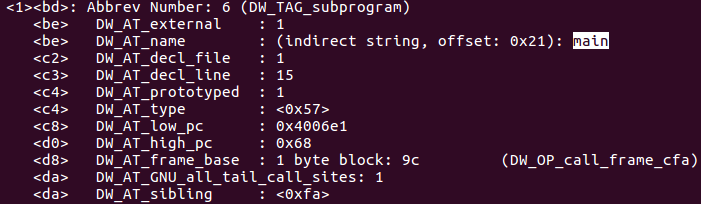
\includegraphics[scale=0.4]{slike/main_subprogram.png}
	\end{center}
	\caption{\texttt{main} funkcija prikazana DWARF potprogramom.}
	\label{fig:mainsub}
\end{figure}

Hardverske tačke prekida su direktno povezane sa hardverom u vidu specijalnih registara. Postavlja se na određenu adresu i hardverski \emph{watchpoint} monitori za zadatu adresu mogu signalizirati razne promene, npr. čitanje, pisanje ili izvršavanje, što im daje prednost u odnosu na softverske tačke prekida. Mane u odnosu na softverske tačke prekida su performanse, koje su neuporedivo sporije, i takođe neophodna hardverska podrška za korišćenje hardverskih tačaka prekida.

\subsection{Koračanje}

Pod procesom koračanja (eng.~\emph{stepping}) kroz program podrazumevamo izvršavanje programa sekvencu po sekvencu. Sekvenca može biti jedna procesorska instrukcija, linija koda ili pak neka funkcija programa koji se debaguje \cite{GDB}.

Instrukcijsko koračanje na platformi Intel x86-64 je direktno omogućeno kroz sistemski poziv \texttt{ptrace}:\newline\newline
\texttt{ptrace(PTRACE\_SINGLESTEP, debuggee\_pid, nullptr, nullptr);}
\newline

Operativni sistem će poslati debageru signal \texttt{SIGTRAP} kada je korak izvršen.

Pored instrukcijkog koračanja pomenućemo još jednu vrstu koračanja u neku funkciju koja je pozvana \texttt{call} ili \texttt{jump} instrukcijom. Komanda debagara GNU GDB koja nam to omogućava jeste \texttt{step in}.

Treba napomenuti da postoje arhitekture za koje ovo ne važi, kao npr. platforma ARM, koja nema hardversku podršku za instrukcijsko koračanje i za njih se koračanje implementira na drugačiji način, uz pomoć emulacije instrukcija, ali u ovom radu neće biti reči o tome.

\subsection{Izlistavanje pozivanih funkcija}

Objasnimo komandu izlistavanje pozivanih funkcija (eng.~\emph{backtrace}) posmatrajući organizaciju stek okvira (eng.~\emph{stack frames}) na platformi Intel x86-64 \cite{GDB}.

\begin{figure}[h!]
	\begin{center}
		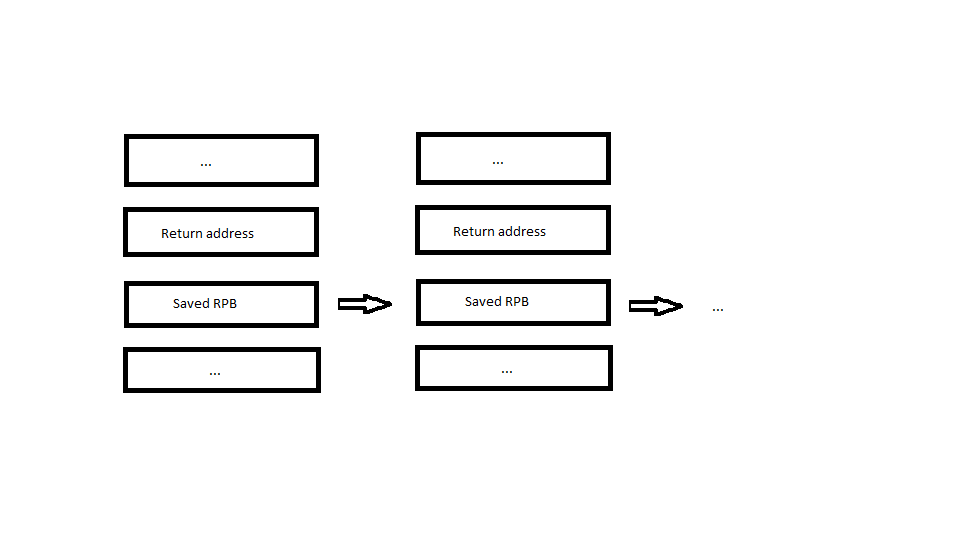
\includegraphics[scale=0.6]{slike/stack_frame.png}
	\end{center}
	\caption{Primer ređanja stek okvira na x86-64 platformi.}
	\label{fig:stack}
\end{figure}

Na slici \ref{fig:stack} navedeni su stek okviri za dva funkcijska poziva. Pre povratne vrednosti funkcije obično se ređaju argumenti funkcije. Sačuvana adresa u registru \texttt{RBP} jeste adresa stek okvira svog pozivaoca. Prateći sve okvire kao elemente povezane liste dolazimo do svih pozivanih funkcija do zadate tačke. Ako se pitamo kako debager ima informaciju o imenu funkcije odgovor je u tome što pretražuje DWARF stablo sa debag informacijama, tražeći \texttt{DW\_TAG\_subprogram} sa odgovarajućom povratnom adresom, pritom čitajući \texttt{DW\_AT\_name} atribut tog elementa.

\subsection{Čitanje vrednosti promenljivih}

Za čitanje vrednosti promenljivih u programu, debager pretražuje DWARF stablo tražeći promenljivu sa zadatim imenom. U slučaju lokalnih promenljivih, traži se \texttt{DW\_TAG\_variable} element čiji \texttt{DW\_AT\_name} odgovara navedenoj promenljivoj. Kada se ista pronađe konsultuje se \texttt{DW\_AT\_location}, koji ukazuje na lokaciju gde se vrednost promenljive nalazi. Ukoliko ovaj atribut nije naveden debager će vrednost takve promenljive smatrati kao optimizovanu prijavljujući informaciju o tome \cite{GDB}.

\chapter{Datoteke jezgra}
\label{chp:corefiles}

Datoteka jezgra (eng.~\emph{core dump file}) je snimak (eng.~\emph{snapshot}) memorije programa, registara i ostalih sistemskih informacija u trenutku neočekivanog prekida rada programa. Veoma važnu ulogu ima u procesu debagovanja programa sa ugrađenih uređaja koji često pripadaju različitoj procesorskoj arhitekturi u odnosu na lični računar. Ugrađeni uređaji obično imaju ograničene resurse, pa nemaju deabger na njoj. Najčešća procedura debagovanja ovakvih programa jeste prebacivanje datoteke jezgra i programa na lični računar na kome se analiza problema dovija koristeći debager.

\section{Struktura datoteke jezgra}

Datoteke jezgra sadrže razne informacije iz memorije programa uključujući i podatke lokalne za niti, vrednosti lokalnih promenljivih, globalnih promenljivih itd. Takođe sadrži vrednosti registara u trenutku prekida programa. U to spadaju i programski brojač i stek pokazivač.

Sadržaj datoteke jezgra je organizovan sekvencijalno sledećim redosledom:

\begin{itemize}
	\item \emph{Zaglavlje}. Sadrži osnovne informacije o datoteci jezgra i ofsete kojima se lociraju ostale informacije iz nje.
	\item \emph{ldinfo strukture}. Definiše informacije relevantne za dinamički loader.
	\item \emph{mstsave strukture}. Definiše informacije relevantne za sistemske niti.
	\item \emph{Korisnički stek}. Sadrži kopiju korisničkog steka u trenutku pucanja programa.
	\item \emph{Segment podataka}. Sadrži kopiju segmenta podataka u trenutku pucanja programa.
	\item \emph{Memorijski mapirani regioni i vm\_info strukture}. Sadrži informacije o ofsetima i dužinama mapiranih regiona.
\end{itemize}

\section{Generisanje datoteke jezgra}

Datoteke jezgra se generišu ukoliko dođe do nepredviđenog prekida programa. To je podrazumevana akcija prilikom okidanja signala operativnog sistema koji ukazuju na prekid rada programa. Jezgra UNIX-olikih operativnih sistema podrazumevano postavljaju dužinu datoteka jezgara na 0. To je razlog zašto na našim sistemima nemamo datoteku jezgra nakon npr.~ prekidanja programa uz poruku \emph{Segmentation fault}. Da bi se datoteke jezgra generisale, potrebno je eksplicitno promeniti dužinu datoteka jezgara koristeći komandu:
\newline
\texttt{ulimit -c unlimited}

Datoteka jezgra se može generisati i iz korisničkog nivoa koristeći GNU GDB alat komandom \texttt{gcore}.

\section{Primer učitavanja datoteke jezgra u GNU GDB alat}

Na slici \ref{fig:ucitavanje_core} prikazan je primer učitavanja datoteke jezgra programa koji čije izvršavanje je prekinuto od strane jezgra operativnog sistema. Komandom alata \texttt{core-file} se učitava datoteka jezgra u debager.

Da bi se izazvalo generisanje datoteke jezgra u izvornom kodu programa napisanog u C ili C++ programskom jeziku može se koristiti \texttt{abort()} funkcija iz standardne C biblioteke. U primieru na slici \ref{fig:ucitavanje_core} je pozvana ta funkcija koja je izazvala prekid programa uz signal \texttt{SIGABRT}. Tom prilikom jezgro operativnog sistema je napravilo datoteku jezgra sa imenom \emph{core}.

\newpage
\begin{figure}[h!]
	\begin{center}
		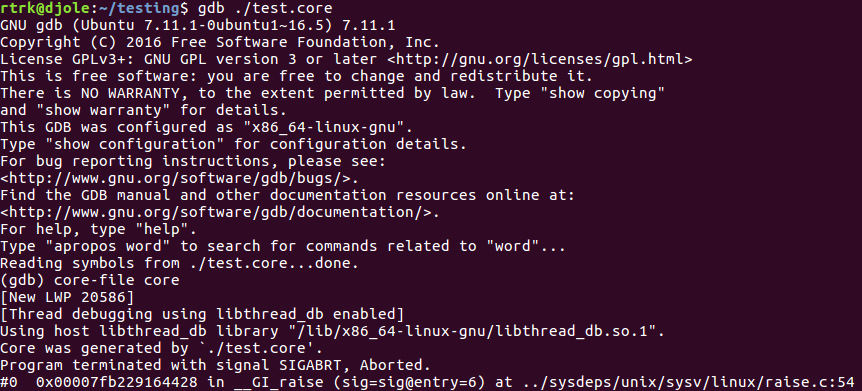
\includegraphics[scale=0.6]{slike/ucitanje_core.png}
	\end{center}
	\caption{Primer učitavanja datoteke jezgra u GNU GDB.}
	\label{fig:ucitavanje_core}
\end{figure}

Na slici \ref{fig:bt_core} je prikazan primer upotrebe komande alata GNU GDB \texttt{bt}. Ona se koristi za izlistavanje pozivanih funkcija programa. Stek okviri programa koji su prikazani na primeru potvrđuju da je u funkciji \texttt{main()} došlo do poziva \texttt{abort()} funkcije. Što je izazvalo prekid rada programa.

\begin{figure}[h!]
	\begin{center}
		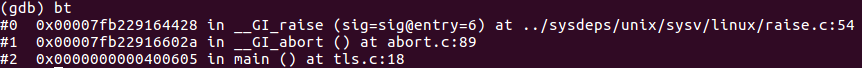
\includegraphics[scale=0.6]{slike/bt_core.png}
	\end{center}
	\caption{Primer izlistavanja pozivanih funkcija koristeći alat GNU GDB uz pomoć datoteke jezgra.}
	\label{fig:bt_core}
\end{figure}

\chapter{Alat GNU GDB}
\label{chp:GDB}

GNU GDB je alat koji nam omogućava da vidimo šta se događa unutar drugog programa dok se izvršava, ili u slučaju neregularnog prekida izvršavanja šta se dešavalo pa je do toga došlo. On nam omogućava da vidimo šta se to dešavalo sa programima i na platformama koje imaju različitu arhitekturu od domaćinske arhitekture. Da bi se to realizovalo koriste se GDB server, što nazivamo udaljeno debagovanje, ili \emph{Multiarch} GNU GDB koji koristi biblioteke namenjene ciljanim arhitekturama. Programi koji mogu biti analizirani mogu biti napisani u raznim programskim jezicima, kao što su Ada, C, C++, Objective-C, Pascal i mnogi drugi. GNU GDB alat se može pokrenuti na najpopularnijim operativnim sistemima UNIX i Microsoft Windows varijanti. U radu se podrazumeva korišćenje UNIX-olikog operativnog sistema.

Poslednja verzija GNU GDB alata koja je realizovana je 8.2.1.

\section{Kako radi GNU GDB?}


\section{Šta je \emph{arhitektura} za GNU GDB?}

Za alat GNU GDB je veoma labav koncept. Može se posmatrati kao bilo koje svojstvo programa koji se debaguje, ali obično se misli na procesorsku arhitekturu. Za debager su bitna dva svojstva procesorske arhitekture:

\begin{itemize}
	\item Skup instrukcija (eng.~\emph{Instruction Set Architecture - ISA}). On predstavlja specifičnu kombinaciju registara i mašinskih instrukcija.
	\item ABI (eng.~\emph{Application Binary Interface}). On predstavlja spisak pravila koja propisuju pravilan način korišćenja skupa instrukcija.
\end{itemize}

\section{Domaćinski GNU GDB}

Domaćinski GNU GDB alat je preveden za istu procesorsku arhitekturu kao i računar na kome se alat izvršava. Korišćenje domaćinskog alata GNU GDB nad nekim programom ima ograničenje. Program koji se debaguje mora biti iste procesorske arhitekture kao i arhitektura domaćina.

\subsection{Prevođenje domaćinskog GNU GDB alata}

Preuzimanje izvornog koda alata se radi sledećim komandama:
\newline
\texttt{mkdir gdb}
\newline
\texttt{cd gdb}
\newline
\texttt{git pull http://gnu.org/gnu/gdb.git}

Prvi korak prevođenja je konfiguracija direktorijuma u kome se prevođenje izvršava. Ovim komandama kreiramo \texttt{Makefile}:
\newline
\texttt{mkdir build}
\newline
\texttt{cd build}
\newline
\texttt{../configure}

Nakon konfiguracije direktorijuma prevođenje alata se vrši komandom:
\newline
\texttt{make}

\subsection{Pokretanje domaćinskog GNU GDB alata}

GNU GDB očekuje kao argument komandne linije program koji je preveden za istu procesorsku arhitekturu kao i on. Pokretanje alata se vrši sledećom komandom:
\newline
\texttt{./gdb/gdb a.out}

\subsection{Korišćenje domaćinskog GNU GDB alata}

Pokažimo neke od osnovnih komandi alata GNU GDB.

\subsubsection{Postavljanje tačke prekida}

Postavljanje tačke prekida na funkciju programa koji se debaguje se vrši komandom \texttt{break}. Primer korišćenja je prikazan na slici \ref{fig:break-fn}. Program koji se debaguje se zaustavlja kada dostigne do određene funkcije.

\begin{figure}[h!]
	\begin{center}
		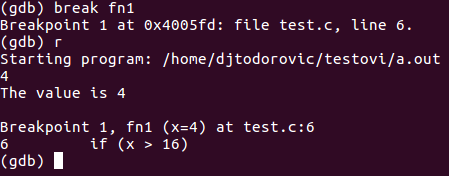
\includegraphics[scale=0.5]{slike/break-fn.png}
	\end{center}
	\caption{Primer postavljanja tačke prekida na funkciju programa.}
	\label{fig:break-fn}
\end{figure}

\subsubsection{Izvršavanje programa sekvencu po sekvencu}

Izvršavanje programa sekvencu po sekvencu se radi pomoću tehnike koračanja. Komanda u okviru alata GNU GDB koja nam omogućava izvršavanje instrukciju po instrukciju je \texttt{stepi}. Primer korišćenja \texttt{stepi} komande, uz pomoć korišćenja \texttt{disassemble} komande koja nam prikazuje asemblerski kod programa koji se debaguje je prikazan na slici \ref{fig:stepi}.

\begin{figure}[h!]
	\begin{center}
		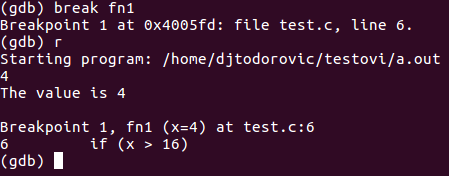
\includegraphics[scale=0.5]{slike/break-fn.png}
	\end{center}
	\caption{Primer izvršavanja pojedinačne instrukcije programa koji se debaguje.}
	\label{fig:stepi}
\end{figure}

Izvršavanje sledeće linije programa se radi korišćenjem komande \texttt{next}. Na slici \ref{fig:next} je prikazan primer korišćenja \texttt{next} komande.

\begin{figure}[h!]
	\begin{center}
		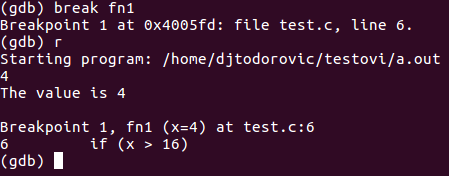
\includegraphics[scale=0.5]{slike/break-fn.png}
	\end{center}
	\caption{Primer izvršavanja sledeće linije programa koji se debaguje.}
	\label{fig:next}
\end{figure}

\newpage
\section{\emph{Multiarch} GNU GDB}

\emph{Multiarch} GNU GDB je verzija alata koja može da debaguje programe sa platformi različitih arhitektura. Alat na korisničkom nivou emulira instrukcije i registre ciljanih platformi. Potrebne su mu i deljene biblioteke za tu ciljanu platformu koje koristi program koji se debaguje. Skup komandi alata je limitiran u odnosu na \emph{domaćinski} GDB.

\subsection{Prevođenje \emph{Multiarch} GNU GDB}

Prvi korak je pozicioniranje u direktorijum sa izvornim kodom alata:
\newline
\texttt{cd gdb}

Prvi korak prevođenja je konfiguracija direktorijuma u kome se prevođenje izvršava. Ovim komandama kreiramo \texttt{Makefile} kojim odobravamo debagovanje svih podržanih arhitektura u alatu GBD (kao npr.~MIPS32, MIPS64, ARM, AARCH64, x86\_64, i386, SPARC i druge):
\newline
\texttt{mkdir build\_multi}
\newline
\texttt{cd build\_multi}
\newline
\texttt{../configure --enable-targets=all}

\subsection{Pokretanje \emph{Multiarch} GNU GDB}

Pokretanje alata \emph{Multiarch} GDB se vrši na isti način kao i domaćinska verzija alata komandom:
\newline
\texttt{./gdb/gdb a.out}

\subsection{Korišćenje \emph{Multiarch} GNU GDB}

Spisak komandi koje se mogu koristiti korišćenjem \emph{Multiarch} verzije alata GNU GDB je limitiran. To se odnosi na izvršavanje programa koji se debaguje, jer pripada program pripada drugačijem adresnom prostoru. Najčešće se ova verzija alata koristi tako što se učita datoteka jezgra koja je generisana na ciljanoj platformi kada je program koji se debaguje neočekivano prekinuo sa radom. To obično prati analiza uzroka greške. Neke od komandi koje mogu biti upotrebljene su izlistavanje vrednosti registara programa, izlistavanje instrukcija, analiza stek okvira pozivanih funkcija, itd.

\subsubsection{Analiza datoteke jezgra}

Na slici \ref{ref:core1} je prikazan primer koristećenja alata \emph{Multiarch} GNU GDB. U primeru se vrši učitavanje datoteke jezgra generisane na ugrađenom uređaju MIPS arhitekture. Uz datoteku jezgra učitavaju se izvršni fajl i deljene biblioteke koje izvršni fajl koristi na ciljanoj platfomi.

\begin{figure}[h!]
	\begin{center}
		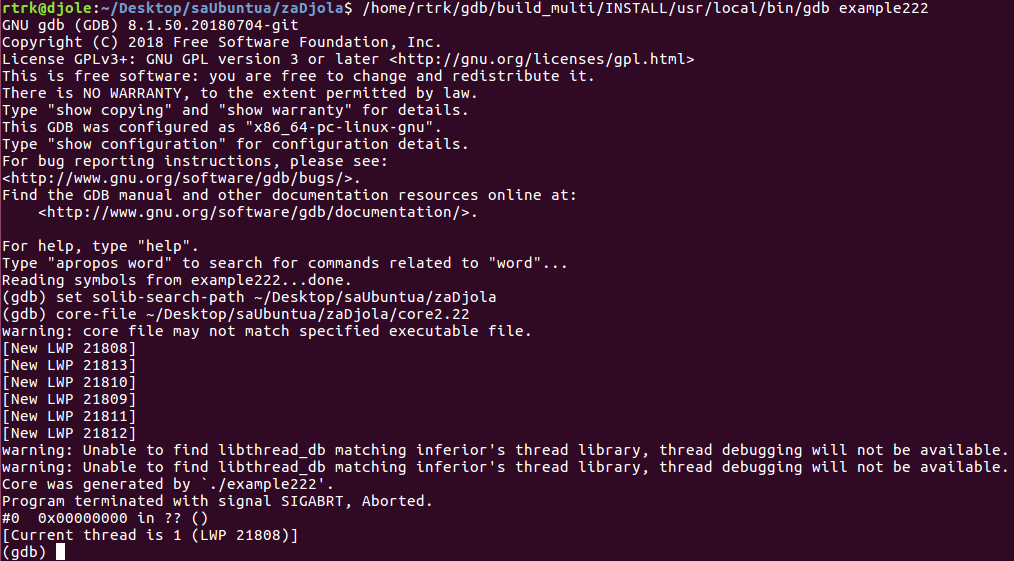
\includegraphics[scale=0.5]{slike/core1.png}
	\end{center}
	\caption{Primer učitavanja datoteke jezgra generisane na MIPS platformi.}
	\label{fig:core1}
\end{figure}

Komanda \texttt{set solib-search-path \emph{dir}} alata GNU GDB korišćena u primeru na sici \ref{ref:core1} služi za navođenje direktorijuma iz kojeg debager treba da koristi deljene biblioteke za učitani program. Ta komanda je veoma bitna za debagovanje programa sa drugih platformi, jer ukoliko putanja nije navedena debager koristi biblioteke na domaćinskoj mašini.

Na primeru sa slike \ref{ref:core2} je prikazana upotreba komande \texttt{info registers}. \emph{Multiarch} GNU GDB čita informaciju o arhitekturi programa koji se debaguje iz datoteke jezgra. Nakon toga čita vrednosti registara iz nje i ispisuje ih.

\begin{figure}[h!]
	\begin{center}
		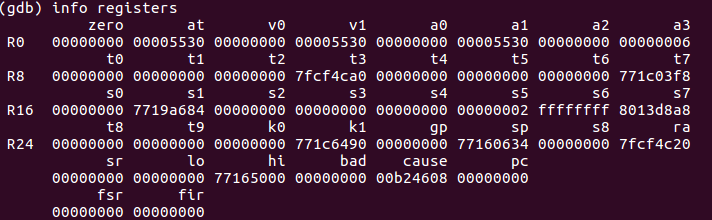
\includegraphics[scale=0.5]{slike/core2.png}
	\end{center}
	\caption{Primer čitanja vrednsoti registara korišćenjem \emph{Multiarch} GNU GDB iz datoteke jezgra generisane na MIPS platformi.}
	\label{fig:core2}
\end{figure}

\chapter{TLS}
\label{chp:TLS}

% ------------------------------------------------------------------------------

\section{Motivacija}
\section{Rukovanje TLS-om tokom izvršavanja programa}
\section{Arhitekturalno specifične zavisnosti}
\section{TLS Modeli pristupa}

\chapter{Implementacija rešenja}
\label{chp:Implementacija}

% ------------------------------------------------------------------------------
\chapter{Zaključak}
% ------------------------------------------------------------------------------

% ------------------------------------------------------------------------------
% Literatura
% ------------------------------------------------------------------------------
\literatura

% ==============================================================================
% Završni deo teze i prilozi
\backmatter
% ==============================================================================

% ------------------------------------------------------------------------------
% Biografija kandidata
\begin{biografija}
\end{biografija}
% ------------------------------------------------------------------------------

\end{document}